\chapter{複素数}%第1章

\begin{mysimplebox}{問1}
$|\alpha+\alpha'|\le|\alpha|+|\alpha'|$
($\alpha,\alpha'\in\C$)を計算によって示せ。
\end{mysimplebox}

$\alpha=a+bi$($a, b\in\R, i=\sqrt{-1}$)に対して$|\alpha|\coloneqq\sqrt{a^2+b^2}$と定義される。

$\alpha'=c+di$($c,d\in\R$)とする。

問1の不等式の左辺について定義に従って変形する。
\begin{align*}
    |\alpha+\alpha'|&=|(a+bi)+(c+di)|\\
    &=|(a+c)+(b+d)i|\\
    &=\sqrt{(a+c)^2+(b+d)^2}
\end{align*}

右辺についても変形する。
\begin{align*}
    |\alpha|+|\alpha'|=\sqrt{a^2+b^2}+\sqrt{c^2+d^2}
\end{align*}

よって、$\sqrt{(a+c)^2+(b+d)^2}\le\sqrt{a^2+b^2}+\sqrt{c^2+d^2}$を示せばよい。

この示すべき目的の式を変形していく。

両辺とも0以上であるから、示すべき式は両辺2
乗した形である以下の式に変形できる。
\begin{align*}
    (a+c)^2+(b+d)^2\le(a^2+b^2)+(c^2+d^2)+2\sqrt{(a^2+b^2)(c^2+d^2)}
\end{align*}

さらに以下のように展開して整理する。
\begin{align}
    (a^2+2ac+c^2)+(b^2+2bd+d^2)&\le (a^2+b^2)+(c^2+d^2)+2\sqrt{(a^2+b^2)(c^2+d^2)}\nonumber\\
    2ac+2bd&\le 2\sqrt{(a^2+b^2)(c^2+d^2)}\nonumber\\
    ac+bd&\le \sqrt{(a^2+b^2)(c^2+d^2)}\label{eq:cauchy-shwarz}\\
    ac+bd&\le \sqrt{a^2c^2+b^2d^2+a^2d^2+b^2c^2}\label{eq:cauchy-shwarz2}
\end{align}
この最終行の不等式(\ref{eq:cauchy-shwarz2})を示せばよいこととなる。

以下の計算をする。
\begin{align}
    &\left(\sqrt{a^2c^2+b^2d^2+a^2d^2+b^2c^2}\right)^2-(ac+bd)^2\nonumber\\
    &=a^2c^2+b^2d^2+a^2d^2+b^2c^2-(a^2c^2+b^2d^2+2abcd)\nonumber\\
    &=a^2d^2+b^2c^2-2abcd\nonumber\\
    &=(ad-bc)^2\ge0\label{eq:togo}
\end{align}
よって、
\begin{align*}
    (ac+bd)^2&\le\left(\sqrt{a^2c^2+b^2d^2+a^2d^2+b^2c^2}\right)^2\\
    |ac+bd|&\le\sqrt{a^2c^2+b^2d^2+a^2d^2+b^2c^2}\\
    ac+bd\le|ac+bd|&\le\sqrt{a^2c^2+b^2d^2+a^2d^2+b^2c^2}
\end{align*}
これで示すべき不等式は示された。

\paragraph{別解}

不等式(\ref{eq:cauchy-shwarz})は、よく知られたコーシー・シュワルツの不等式である。すなわち、$\bm{x}=(a,b)$、$\bm{y}=(c,d)$とすると、不等式(\ref{eq:cauchy-shwarz})は、ベクトルの内積と大きさによって、
\begin{align}
    \bm{x}\cdot \bm{y}\le|\bm{x}||\bm{y}|\label{eq:cauchy-shwarz0}
\end{align}
と書き表される。

この不等式は、$t\in\R$に対して、以下のよく知られた証明がある。すなわち、
\begin{align*}
    0\le|t\bm{x}+\bm{y}|^2
    =|\bm{x}|^2t^2+2(\bm{x}\cdot\bm{y})t+|\bm{y}|^2
\end{align*}
であるが、2次方程式$|\bm{x}|^2t^2+2(\bm{x}\cdot\bm{y})t+|\bm{y}|^2=0$の判別式$D\le 0$より
\begin{align*}
    \frac{D}{4}=(\bm{x}\cdot\bm{y})^2-|\bm{x}|^2|\bm{y}|^2\le 0
\end{align*}
よって、$\bm{x}\cdot\bm{y}\le|\bm{x}\cdot\bm{y}|\le|\bm{x}||\bm{y}|$が言える。

\begin{mysimplebox}{問2}
    $z_k\in\C$($k=1,2,\dots,n$)に対して、$|z_1+z_2+\dots+z_n|\le|z_1|+|z_2|+\dots+|z_n|$であり、等号が成立するのは、$z_k$($k=1,2,\dots,n$)が$z=0$を起点とする同じ半直線の上にあるときに限ることを示せ。
\end{mysimplebox}

$|z_1+z_2+\dots+z_n|\le|z_1|+|z_2|+\dots+|z_n|$であることは、問1の結果と$n$に関する帰納法によって示される。

$n=2$のとき、等号が成立する条件を考える。すなわち、$|z_1+z_2|=|z_1|+|z_2|$が成り立っているとする。複素数と実2次元平面上の点を同一視して$z_1=(a,b), z_2=(c,d)$($a,b,c,d\in\R$)とすると、($\ref{eq:togo}$)式より、$ad=bc$の場合に限られることが分かる。

$a=0$の場合、$b=0$または$c=0$である。

$b=0$の場合、$z_1=(0,0)$であるから、どのような$z_2=(c,d)$に対しても$z_1, z_2$は原点を起点とする半直線上にある。

$c=0$の場合、$z_1=(0,b), z_2=(0,d)$であるが、$|z_1+z_2|=|z_1|+|z_2|$は、
\begin{align*}
    |b+d|=|b|+|d|
\end{align*}
と書き直される。これは$b$と$d$が同符号であることを表す。よって$z_1$と$z_2$は虚軸上で同じ方向を向いており、原点を起点とする半直線上にあることが分かる。

$a\neq 0$の場合、($\ref{eq:togo}$)式より、$c\neq 0$であり、次の式が成り立つ。
\begin{align*}
    \frac{b}{a}=\frac{d}{c}=k
\end{align*}
これは、$z_1$と$z_2$が同一直線上にあることを表している。

さらに、
\begin{align*}
    |z_1+z_2|&=|(a+c)+(b+d)i|\\
    &=|(a+c)+(ak+ck)i|\\
    &=|a+c||1+ki|\\
    &=|a+c|\sqrt{1+k^2}\\
    |z_1|+|z_2|&=|a+bi|+|c+di|\\
    &=|a+aki|+|c+cki|\\
    &=|a||1+ki|+|c||1+ki|\\
    &=(|a|+|c|)\sqrt{1+k^2}
\end{align*}
よって、$|a+c|=|a|+|c|$が成り立つ。これは$a$と$c$が同符号であることを表している。

以上より、$z_1$と$z_2$は原点を起点とする半直線上にある。

逆に、$z_1$と$z_2$は原点を起点とする半直線上にあるとき、問題の不等式の等号が成立している。

したがって、$n=2$のとき、不等式の等号が成立するのは$z_1$と$z_2$が原点を起点とする半直線上にあることが示せた。

$n=3$以上のときも、帰納法によって示される。

ところで、($\ref{eq:cauchy-shwarz0}$)式において、$\bm{x}\cdot \bm{y}=|\bm{x}||\bm{y}|\cos \theta$(ただし$\theta$は$z_1$と$z_2$のなす角の大きさ)であることを知っていれば、問題の不等式の等号が成り立つのは、$|\bm{x}||\bm{y}|\cos \theta=|\bm{x}||\bm{y}|$のときであり、$\bm{x}, \bm{y}$ともに0でなければ$\cos \theta=1$となる。よって、$\theta=0$($2\pi$分の違いは無視する)であるから、不等式の等号が成立するのは、複素数平面上の点たちが原点を起点とする半直線上にあることが容易に分かる。

\begin{mysimplebox}{問3}
    $|\alpha|<1$のとき、$|z|<1$ならば$\left|\frac{z-\alpha}{\bar{\alpha}z-1}\right|<1$であり、$|z|=1$ならば$\left|\frac{z-\alpha}{\bar{\alpha}z-1}\right|=1$であることを示せ。
\end{mysimplebox}

$\alpha=a+bi, z=c+di$($a,b,c,d\in\R$)とする。

\begin{align*}
    |\bar{\alpha}z-1|&=|(a-bi)(c+di)-1|\\
    &=|(ac+bd-1)+(ad-bc)i|\\
    &=\sqrt{(ac+bd-1)^2+(ad-bc)^2}\\
    &=\sqrt{(a^2c^2+b^2d^2+1+2abcd-2bd-2ac)+(a^2d^2-2abcd+b^2c^2)}\\
    &=\sqrt{a^2c^2+b^2d^2-2bd-2ac+a^2d^2+b^2c^2+1}\\
    &=\sqrt{(a^2+b^2)(c^2+d^2)-2(ac+bd)+1}\\
    |z-\alpha|&=|(c-a)+(d-b)i|\\
    &=\sqrt{(c-a)^2+(d-b)^2}\\
    &=\sqrt{a^2+b^2+c^2+d^2-2(ac+bd)}
\end{align*}
よって、
\begin{align*}
    &|\bar{\alpha}z-1|^2-|z-\alpha|^2\\
    =&(a^2+b^2)(c^2+d^2)-(a^2+b^2)-(c^2+d^2)+1\\
    =&\{(a^2+b^2)-1\}\{(c^2+d^2)-1\}
\end{align*}

$|\alpha|<1$ならば$(a^2+b^2)-1<0$、$|z|<1$ならば$(c^2+d^2)-1<0$である。
よって、
\begin{align*}
    &|\bar{\alpha}z-1|^2-|z-\alpha|^2>0\\
    &|\bar{\alpha}z-1|^2>|z-\alpha|^2\\
    &|\bar{\alpha}z-1|>|z-\alpha|\\
    &\left|\frac{z-\alpha}{\bar{\alpha}z-1}\right|<1
\end{align*}

また、$|z|=1$ならば$(c^2+d^2)-1=0$であるから、上記と同じ計算で等号が成り立ち、
\begin{align*}
    &\left|\frac{z-\alpha}{\bar{\alpha}z-1}\right|=1
\end{align*}
が言える。

\paragraph{別解1}

図形的に解くこともできる。

$\arg\bar{\alpha}z-\arg 1=\arg\bar{\alpha}+\arg z-0=-\arg\alpha+\arg z$であるから、3点$\bar{\alpha}z$,O,1がなす角度と、3点$z$,O,$\alpha$がなす角度は等しい。その大きさを$\theta$とすると、余弦定理により、
\begin{align*}
    |z-\alpha|^2&=|z|^2+|\alpha|^2-2\cos\theta\\
    |\bar{\alpha}z-1|^2&=|\bar{\alpha}z|^2+1^2-2|\bar{\alpha}z|\cos\theta\\
    &=|\alpha|^2|z|^2+1-2|\bar{\alpha}z|\cos\theta
\end{align*}
よって、
\begin{align*}
    |\bar{\alpha}z-1|^2-|z-\alpha|^2&=|\alpha|^2|z|^2-|z|^2-|\alpha|^2+1\\
    &=(|z|^2-1)(|\alpha|^2-1)
\end{align*}
ゆえに、$|\alpha|<1, |z|<1$のとき、 $|\bar{\alpha}z-1|^2-|z-\alpha|^2>0$となり、上記と同じ結論を得る。

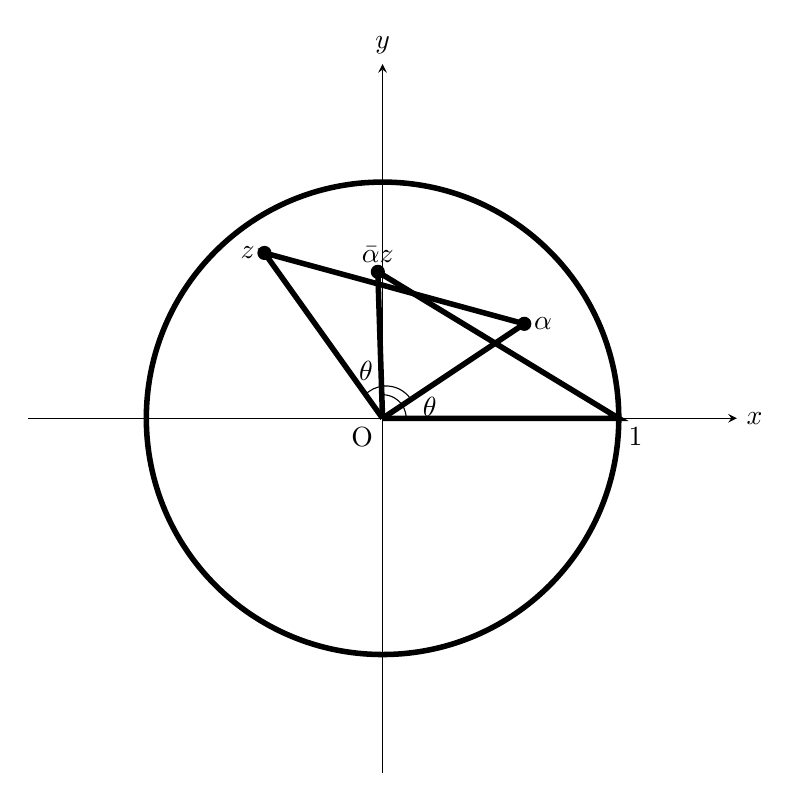
\begin{tikzpicture}[x=30mm,y=30mm,domain=-1.5:1.5,samples=200,>=stealth]
    \draw[->](-1.5,0)--(1.5,0) node[right]{$x$};
    \draw[->](0,-1.5)--(0,1.5) node[above]{$y$};
    \draw (0,0) node[below left]{O};
    \draw[line width=2pt] (0,0) circle (1);
    \fill[black] (-0.5,0.7) circle (0.03) node[left] {$z$}
                 (0.6,0.4) circle (0.03) node[right] {$\alpha$}
                 (-0.02,0.62) circle (0.03) node[above]{$\bar{\alpha}z$};
    \draw (1,0) node[below right] {1};
    \draw[line width=2pt] (0,0)--(-0.5,0.7)--(0.6,0.4)--(0,0);
    \draw[line width=2pt] (0,0)--(-0.02,0.62)--(1,0)--(0,0);
    \draw (0.1,0) arc (0:92:0.1);
    \draw (0.2,0.05) node {$\theta$};
    \draw (0.12,0.08) arc (33:138:0.125);
    \draw (-0.07,0.2) node {$\theta$};
\end{tikzpicture}

\paragraph{別解2}
複素数の計算規則によって、
\begin{align*}
    |\bar{\alpha}z-1|^2-|z-\alpha|^2
    &=(\bar{\alpha}z-1)(\alpha\bar{z}-1)-(z-\alpha)(\bar{z}-\bar{\alpha})\\
    &=|\alpha|^2|z|^2-\bar{\alpha}z-\alpha\bar{z}+1-(|z|^2-\bar{\alpha}z-\alpha\bar{z}+|\alpha|^2)\\
    &=|\alpha|^2|z|^2-|z|^2-|\alpha|^2+1\\
    &=(|z|^2-1)(|\alpha|^2-1)
\end{align*}
と計算でき、上記と同様の結論を得る。

\begin{mysimplebox}{問4(Cauchy--Hadamard)}
    $\sum_{n=0}^\infty c_nz^n=c_0+c_1z+\dots+c_nz^n+\dots$(①)の形の級数を$z$の\textgt{整級数}という。
    \[\overline{\lim_{n\to\infty}}|c_n|^{\frac{1}{n}}=\left\{\begin{array}{lll}
      \lambda  \,(0<\lambda<+\infty) & \mbox{ならば} & R=\frac{1}{\lambda}\\
      0 & \mbox{ならば} & R=+\infty\\
      +\infty & \mbox{ならば} & R=0
    \end{array}\right.\]
    として$R$を定めるとき、$\sum_{n=0}^\infty c_nz^n$は$|z|<R$ならば絶対収束し、$|z|>R$ならば発散する。このことを示せ。
\end{mysimplebox}
\paragraph{証明}
$0<\lambda<+\infty$の場合は本で証明が済んでいるので省略する。

まずは$\displaystyle\overline{\lim_{n\to\infty}}|c_n|^{\frac{1}{n}}=0$のときを考える。整級数①が$|z|<+\infty$で絶対収束することを示せばよい。

$|z|<\frac{1-\delta}{\delta}$を満たす$\delta\,(0<\delta<1)$が存在する。

$\displaystyle\overline{\lim_{n\to\infty}}|c_n|^{\frac{1}{n}}=0$であるから、十分大きい$n$に対して$|c_n|^\frac{1}{n}<\delta$となる。

よって、
\begin{align*}
    |c_nz^n|&=\left(|c_n|^\frac{1}{n}\right)^n|z|^n<\delta^n\left(\frac{1-\delta}{\delta}\right)^n
    =(1-\delta)^n.
\end{align*}
ゆえに、
\begin{align*}
    \sum_{k=n}^\infty |c_kz^k|&<\sum_{k=n}^\infty(1-\delta)^k
\end{align*}
$0<1-\delta<1$であるから、上式の左辺は等比級数として収束する。したがって、$\sum_{k=n}^\infty |c_kz^k|$も収束する。すなわち、整級数①は絶対収束する。

次に$\displaystyle\overline{\lim_{n\to\infty}}|c_n|^{\frac{1}{n}}=+\infty$のときを考える。

$|z|>0$ならば整級数①が発散することを示せばよい。

$|z|>0$とすると、$|z|>\frac{1}{\delta}>0$となる$\delta\,(>0)$が存在する。

十分大きい$n$に対して、$|c_n|^\frac{1}{n}>\delta$が成り立つ。

よって、
\begin{align*}
    |c_nz^n|&=\left(|c_n|^\frac{1}{n}\right)^n|z|^n>\delta^n\left(\frac{1}{\delta}\right)^n
    =1.
\end{align*}
ゆえに、$|c_nz^n|\to 0$でないため、整級数①は発散する。(証明終)

この問題からも分かったことだが、級数の収束の判定法の1つは、等比級数と比較することである。

上記で定めた$R$を整級数①の\textgt{収束半径}という。


\begin{mysimplebox}{問5}
    $\sum_{n=0}^\infty c_nz^n$が$z=z_0$で収束すれば$|z|<|z_0|$であるような$z$に対しては絶対収束することを示せ。
\end{mysimplebox}
\paragraph{証明}
本にも書いてあるとおり、これは言い換えると、「$\sum_{n=0}^\infty c_nz^n$が$z=z_1$で絶対収束しなければ$|z|>|z_1|$であるような$z$に対しては発散する」ということである。この言い換えた方を示す。

$\sum_{n=0}^\infty c_nz^n$が$z=z_1$で絶対収束しなければ、収束半径$R$は、$R<|z_1|$である。よって、$|z|>|z_1|>R$では、$\sum_{n=0}^\infty c_nz^n$は発散する。(証明終)

\begin{mysimplebox}{問6}
    $c_n\neq 0\,(n=k, k+1, k+2,\dots)$、$R=\lim_{n\to\infty}|c_nc_{n+1}^{-1}|$ならば、$\sum_{n=0}^\infty c_nz^n$の収束半径は$R$である。
\end{mysimplebox}
\paragraph{証明}
$R=\lim_{n\to\infty}|c_nc_{n+1}^{-1}|$であることより、$0<\epsilon<R$である任意の数$\epsilon$に対して、ある正数$N$が存在し、$n>N$となる任意の$n$に対して、
\begin{align*}
    R-\epsilon<\left|\frac{c_n}{c_{n+1}}\right|<R+\epsilon
\end{align*}
となる。よって、
\begin{align*}
    \frac{|c_n|}{R+\epsilon}<|c_{n+1}|<\frac{|c_n|}{R-\epsilon}
\end{align*}    
である。

ゆえに、$k>0$に対して、
\begin{align}
    |c_{n+k}|&>\frac{|c_{n+k-1}|}{R+\epsilon}>\frac{|c_{n+k-2}|}{(R+\epsilon)^2}>\dots>\frac{|c_{n}|}{(R+\epsilon)^k},\label{eq:convR1}\\
    |c_{n+k}|&<\frac{|c_{n+k-1}|}{R-\epsilon}<\frac{|c_{n+k-2}|}{(R-\epsilon)^2}<\dots<\frac{|c_{n}|}{(R-\epsilon)^k}.\label{eq:convR2}
\end{align}

したがって、
\begin{align*}
    \left\{\frac{|c_{n}|}{(R+\epsilon)^k}\right\}^\frac{1}{n+k}<&|c_{n+k}|^\frac{1}{n+k}< \left\{\frac{|c_{n}|}{(R-\epsilon)^k}\right\}^\frac{1}{n+k}\\
    \frac{|c_{n}|^\frac{1}{n+k}}{(R+\epsilon)^\frac{k}{n+k}}<&|c_{n+k}|^\frac{1}{n+k}< \frac{|c_{n}|^\frac{1}{n+k}}{(R-\epsilon)^\frac{k}{n+k}}
\end{align*}
ここで、$k\longrightarrow\infty$の極限において、
\begin{align*}
    \frac{|c_{n}|^\frac{1}{n+k}}{(R+\epsilon)^\frac{k}{n+k}}&\longrightarrow \frac{|c_{n}|^0}{(R+\epsilon)^1}=\frac{1}{R+\epsilon},\\
    \frac{|c_{n}|^\frac{1}{n+k}}{(R-\epsilon)^\frac{k}{n+k}}&\longrightarrow \frac{|c_{n}|^0}{(R-\epsilon)^1}=\frac{1}{R-\epsilon}.
\end{align*}
よって、
\begin{align*}
    \frac{1}{R+\epsilon}<\lim_{k\to\infty}|c_{n+k}|^\frac{1}{n+k}<\frac{1}{R-\epsilon}.
\end{align*}
$\epsilon$はいくらでも小さくとれるから、
\begin{align*}
    \lim_{k\to\infty}|c_{n+k}|^\frac{1}{n+k}=\frac{1}{R}
\end{align*}
したがって、Cauchy--Hadamardの定理により、$\sum_{n=0}^\infty c_nz^n$の収束半径は$R$である。(証明終)

\paragraph{別解}
Cauchy--Hadamardの定理を使わず、$R$が収束半径であることを直接示す。

$0<\epsilon<\frac{R}{2}$である$\epsilon$に対して、$(\ref{eq:convR1}),(\ref{eq:convR2})$式が成り立っているとする。

まずは$|z|<R-2\epsilon$のときを考える。
$(\ref{eq:convR2})$式から、
\begin{align*}
    \sum_{k=0}^\infty |c_{n+k}z^{n+k}|
    <\sum_{k=0}^\infty \frac{|c_n|(R-2\epsilon)^{n+k}}{(R-\epsilon)^k}=|c_n|(R-2\epsilon)^n\sum_{k=0}^\infty \left(\frac{R-2\epsilon}{R-\epsilon}\right)^k
\end{align*}
$0<\frac{R-2\epsilon}{R-\epsilon}<1$であるから、$\sum_{n=0}^\infty c_nz^n$は絶対収束する。

次に$|z|>R+2\epsilon$のときを考える。
$(\ref{eq:convR1})$式から、
\begin{align*}
    \sum_{k=0}^\infty |c_{n+k}z^{n+k}|
    >\sum_{k=0}^\infty \frac{|c_n|(R+2\epsilon)^{n+k}}{(R+\epsilon)^k}=|c_n|(R+2\epsilon)^n\sum_{k=0}^\infty \left(\frac{R+2\epsilon}{R+\epsilon}\right)^k
\end{align*}
$1<\frac{R+2\epsilon}{R+\epsilon}$であるから、$\sum_{n=0}^\infty c_nz^n$は発散する。

よって、$\sum_{n=0}^\infty c_nz^n$の収束半径$r$は、$R-2\epsilon<r<R+2\epsilon$を満たす。$\epsilon$は$0<\epsilon<\frac{R}{2}$の範囲で任意であるから、$r=R$である。(証明終)